% Provenance (never printed): cycle 2 "Questionner le monde de la matiere"
% (solid materials, observing and sorting) and cycle 3 theme 4 (local geology,
% rocks for building); see sources/book1/PROVENANCE.md. Book 1, grade 3, ch. 1.
\chapter{石头、卵石和沙}\label{ch:g3:stones-pebbles-sand}

汤姆在河边度假。在\omterm{def:g3:stones-pebbles-sand:pebble}{砾石}滩上，那里的水很
浅，他捡起一块\omterm{def:g3:stones-pebbles-sand:pebble}{卵石}。它光滑而圆，几乎像一枚卵，
并且正好能握在手里。上周，他和父母在山间
小路上行走，在同一\omterm{def:g1:landscapes-around-us:landform}{山谷}高处，他看到颜色相同的石头躺在
一处\omterm{def:g3:stones-pebbles-sand:rock}{岩石}坡下——但那些石头很尖锐，有棱有角。

山上的一块尖石头，是怎样在\omterm{def:g1:landscapes-around-us:landform}{山谷}下游
变成光滑圆润的\omterm{def:g3:stones-pebbles-sand:pebble}{卵石}的呢？要弄清这个问题，先从\omterm{def:g3:stones-pebbles-sand:rock}{岩石}本身说起。

\begin{omfigure}
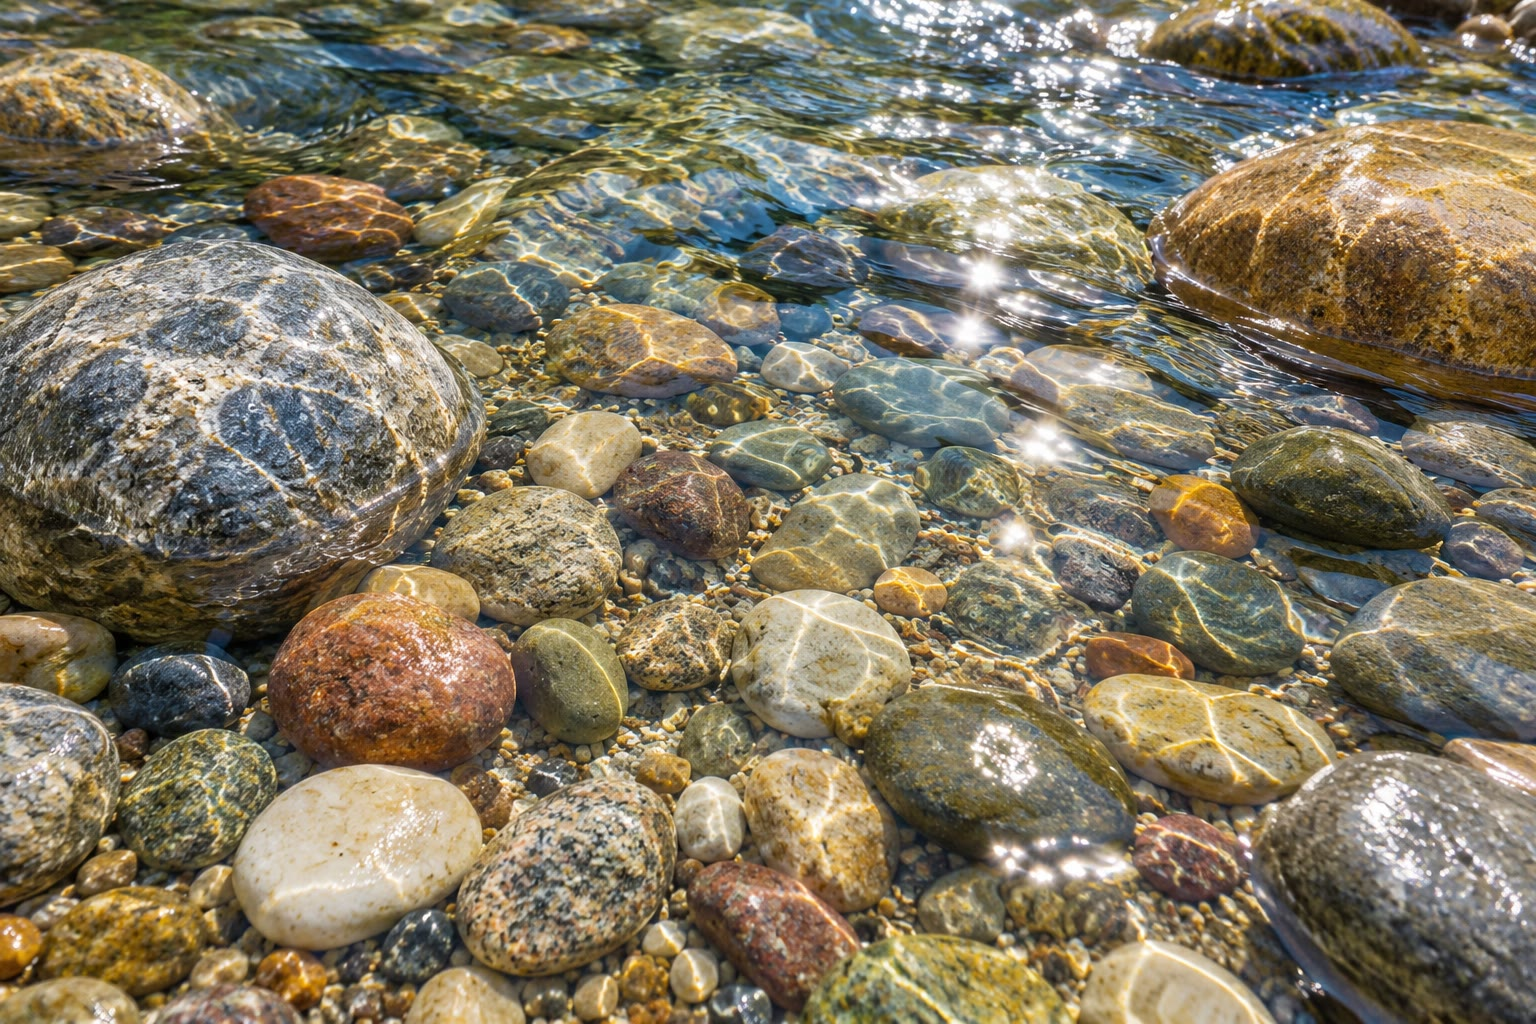
\includegraphics[width=0.62\linewidth]{images/book1/ai/g3-stream-pebbles.jpg}

{\small 溪流澄清的水下，是一颗颗圆形的\omterm{def:g3:stones-pebbles-sand:pebble}{卵石}。}
\end{omfigure}

\begin{recall}
\omterm{def:g1:landscapes-around-us:landscape}{景观}中有山、\omterm{def:g1:landscapes-around-us:landform}{丘陵}、\omterm{def:g1:landscapes-around-us:landform}{山谷}和\omterm{def:g1:landscapes-around-us:landform}{平原}，还有
从高地流入大海的\omterm{def:g1:landscapes-around-us:water}{河流}
（见\cref{ch:g1:landscapes-around-us}）。地面最上层是土壤，
也就是植物生长的地方。生物课本会告诉我们，
生物是如何形成土壤的。
\end{recall}

\section{岩石：脚下坚硬的大地}

在花园里挖一个深坑。先看到深色、松软的土壤，
里面夹着树根。往下，土壤颜色变浅，石头更多。若挖得足够深，
就一定会碰到铁锹挖不动的坚硬东西：
\omterm{def:g3:stones-pebbles-sand:rock}{岩石}。

\begin{definition}[岩石与基岩]\label{def:g3:stones-pebbles-sand:rock}
\emph{岩石}\index{岩石}是构成固体地球的一种坚硬天然材料。
\emph{基岩}\index{基岩}是指位于
陆地各处土壤之下、海底沙与泥之下的
固体岩石。
\end{definition}

大多数地方，\omterm{def:g3:stones-pebbles-sand:rock}{基岩}被土壤、草和树木覆盖着。
只有在没有土壤覆盖的地方我们才能看到它，比如
陡峭的山坡上、海边的悬崖上，以及
穿过山丘开凿出来的道路旁。

\begin{omfigure}
\begin{tikzpicture}[x=1cm, y=1cm, font=\small]
  % bedrock
  \fill[omLithGranite!60] (0,0) rectangle (11,2.2);
  \foreach \x/\y in {0.6/0.5, 1.8/1.4, 3.1/0.7, 4.4/1.6, 5.6/0.4, 6.9/1.2, 8.3/0.6, 9.6/1.5, 10.3/0.4}
    \draw[black!40, line width=0.4pt] (\x,\y) -- ++(0.5,0.25);
  % soil (thick on the left, missing on the steep right)
  \fill[brown!55] (0,2.2) -- (0,3.4) .. controls (2,3.5) and (4,3.4) .. (5.6,3.2) -- (6.4,2.9) -- (6.4,2.2) -- cycle;
  \fill[brown!30] (0,2.2) rectangle (6.4,2.65);
  % rock showing on the right: a hill side with no soil
  \fill[omLithGranite!60] (6.4,2.2) -- (6.4,2.9) -- (7.6,3.9) -- (8.8,4.3) -- (11,4.3) -- (11,2.2) -- cycle;
  \draw[black!60] (0,3.4) .. controls (2,3.5) and (4,3.4) .. (5.6,3.2) -- (6.4,2.9) -- (7.6,3.9) -- (8.8,4.3) -- (11,4.3);
  % grass and roots
  \foreach \x in {0.3,0.8,...,5.3}
    \draw[green!50!black, line width=0.6pt] (\x,{3.4-0.04*\x}) -- ++(0.05,0.18);
  \foreach \x in {1.2,3.4,4.9}
    \draw[brown!80!black, line width=0.5pt] (\x,3.3) -- ++(-0.1,-0.5) -- ++(0.15,-0.3);
  % labels
  \node[anchor=west] at (11.2,3.6) {露出的岩石};
  \node[anchor=west] at (11.2,3.2) {地表};
  \draw[black!60] (11.15,3.4) -- (9.6,4.15);
  \node[anchor=east] at (-0.2,2.9) {土壤};
  \draw[black!60] (-0.15,2.9) -- (0.6,2.9);
  \node[anchor=west] at (11.2,1.1) {基岩};
  \draw[black!60] (11.15,1.1) -- (10.6,1.1);
\end{tikzpicture}

{\small 地面剖面图。土壤之下总是坚硬的
\omterm{def:g3:stones-pebbles-sand:rock}{基岩}。在右侧陡峭的山坡上，土壤缺失，
\omterm{def:g3:stones-pebbles-sand:rock}{岩石}露出了地表。}
\label{fig:g3:stones-pebbles-sand:ground}
\end{omfigure}

\section{从岩石到卵石}

\omterm{def:g3:stones-pebbles-sand:rock}{岩石}虽然坚硬，却并非永恒不变。冬天，水进入
\omterm{def:g3:stones-pebbles-sand:rock}{岩石}的裂缝中，凝固膨胀，把裂缝撑得更大。
植物的根也会长进裂缝里。日积月累，碎块断裂脱落，
山坡下那些尖锐的石头就是这样来的。

尖锐的石头落入山间溪流后，水流便把它沿河底滚动，
撞击其他石块，并拖着它越过沙地。它的
棱角最先被磨掉。石头走得越远，就越圆、
越光滑。等它到达\omterm{def:g1:landscapes-around-us:landform}{山谷}下游时，已经
变成了\omterm{def:g3:stones-pebbles-sand:pebble}{卵石}。

\begin{definition}[卵石与砾石]\label{def:g3:stones-pebbles-sand:pebble}
\emph{卵石}\index{卵石}是一小块\omterm{def:g3:stones-pebbles-sand:rock}{岩石}，经过
水流在河中或海滩上的滚动而磨圆、磨光。
\emph{砾石}\index{砾石}是由许多小石块和卵石堆积在一起，
颗粒比\omterm{def:g3:stones-pebbles-sand:sand}{沙粒}大。
\end{definition}

\begin{omfigure}
\begin{tikzpicture}[x=1cm, y=1cm, font=\small]
  \draw[ocBlue!70!black, line width=1.2pt, -{Stealth[length=3mm]}] (0,0) -- (12.2,0);
  \node[below, font=\scriptsize] at (6.1,-0.15) {溪流把石头带向下游，每次洪水都会带得更远一点};
  \foreach \x/\shape/\t in {
     0.8/{(-0.55,-0.1) -- (-0.2,0.5) -- (0.35,0.55) -- (0.6,0.05) -- (0.3,-0.45) -- (-0.35,-0.5) -- cycle}/从岩石上脱落, 
     4.0/{(-0.5,-0.1) [rounded corners=4pt] -- (-0.2,0.45) -- (0.3,0.5) -- (0.55,0.05) -- (0.3,-0.4) -- (-0.35,-0.45) -- cycle}/棱角被磨圆, 
     7.2/{(-0.45,-0.05) [rounded corners=8pt] -- (-0.15,0.42) -- (0.3,0.45) -- (0.5,0.05) -- (0.3,-0.35) -- (-0.3,-0.4) -- cycle}/{更圆、更小}, 
     10.4/{(0,0) ellipse (0.45 and 0.3)}/一颗光滑的卵石} {
    \begin{scope}[shift={(\x,1.1)}]
      \fill[omLithGranite!80, draw=black!70] \shape;
    \end{scope}
    \node[font=\scriptsize] at (\x,0.35) {\t};
  }
\end{tikzpicture}

{\small 石头在河中的旅程：刚从\omterm{def:g3:stones-pebbles-sand:rock}{岩石}上掉下时棱角尖锐，
经过长途顺流而下后变得圆润光滑。}
\label{fig:g3:stones-pebbles-sand:journey}
\end{omfigure}

\begin{remark}[读懂石头的形状]\label{rem:g3:stones-pebbles-sand:shape}
石头的形状讲述着它的故事。棱角分明的石头
离它所断裂的\omterm{def:g3:stones-pebbles-sand:rock}{岩石}并不远；圆润光滑的\omterm{def:g3:stones-pebbles-sand:pebble}{卵石}
则在\omterm{def:g1:landscapes-around-us:water}{河流}或海浪中被水长时间滚动过。
\end{remark}

\section{沙和泥}

石头和\omterm{def:g3:stones-pebbles-sand:pebble}{卵石}相互碰撞，也会剥落下细小的
碎屑。经过极长的时间，这些细小碎屑变成\omterm{def:g3:stones-pebbles-sand:sand}{沙子}。用放大镜看\omterm{def:g3:stones-pebbles-sand:sand}{沙子}：
每一粒沙都是一小块\omterm{def:g3:stones-pebbles-sand:rock}{岩石}，或是一小块
贝壳的碎片，通常也是圆的。

\begin{definition}[沙和泥]\label{def:g3:stones-pebbles-sand:sand}
% ledger: usgs:wentworth
\emph{沙}\index{沙}是由直径小于
2 毫米的碎岩屑颗粒构成的，仍能看清每一粒。\emph{泥}\index{泥}是
由细小到无法逐粒看清的颗粒组成；湿润时，它
柔软而黏。
\end{definition}

地质学家按大小对碎岩块进行分类，从最大到
最小依次为：巨砾、\omterm{def:g3:stones-pebbles-sand:pebble}{卵石}和\omterm{def:g3:stones-pebbles-sand:pebble}{砾石}、沙和泥。

\begin{omfigure}
\begin{tikzpicture}[x=1mm, y=1mm, font=\small]
  % true size: 1 unit = 1 mm
  \draw[black!40] (0,-14) -- (150,-14);
  \foreach \x in {0,10,...,150} \draw[black!40] (\x,-14) -- (\x,-12.5);
  \foreach \x in {0,50,100,150} \node[font=\scriptsize, below] at (\x,-14.5) {\pgfmathparse{int(\x/10)}\pgfmathresult\,厘米};
  % mud: too small
  \node[font=\scriptsize, align=center] at (6,14) {泥};
  \fill[brown!60] (6,0) circle (0.05);
  \node[font=\scriptsize, align=center] at (6,4.5) {颗粒小到 \\看不见};
  % sand grains: up to 2 mm
  \node[font=\scriptsize] at (28,14) {沙};
  \foreach \x/\r in {22/0.3, 25/0.5, 28/0.75, 32/1.0}
    \fill[yellow!60!brown, draw=black!50, line width=0.2pt] (\x,0) circle (\r);
  \node[font=\scriptsize, align=center] at (28,5) {小于 \\2 毫米};
  % gravel and pebbles
  \node[font=\scriptsize] at (78,22) {砾石和卵石};
  \fill[omLithGranite!80, draw=black!60] (52,0) ellipse (2 and 1.5);
  \fill[black!25, draw=black!60] (62,0) ellipse (4 and 3);
  \fill[omLithGranite!80, draw=black!60] (78,0) ellipse (8 and 6);
  \fill[black!30, draw=black!60] (104,0) ellipse (15 and 10);
  % boulder: off scale
  \node[font=\scriptsize] at (138,22) {巨砾};
  \fill[black!20, draw=black!60] (128,-10) .. controls (127,8) and (135,16) .. (142,15) .. controls (150,14) and (152,4) .. (149,-10) -- cycle;
  \node[font=\scriptsize, align=center, fill=white, fill opacity=0.7, text opacity=1, inner sep=1pt] at (139,4) {画得 \\太小了};
\end{tikzpicture}

{\small 碎岩屑颗粒，从最小到最大。泥、沙、
\omterm{def:g3:stones-pebbles-sand:pebble}{砾石}和\omterm{def:g3:stones-pebbles-sand:pebble}{卵石}均按实际大小绘制，可以用尺子比一比。一
块巨砾可以和一把椅子一样大，也可能像一幢房子那么大。}
\label{fig:g3:stones-pebbles-sand:sizes}
\end{omfigure}

\begin{omfigure}
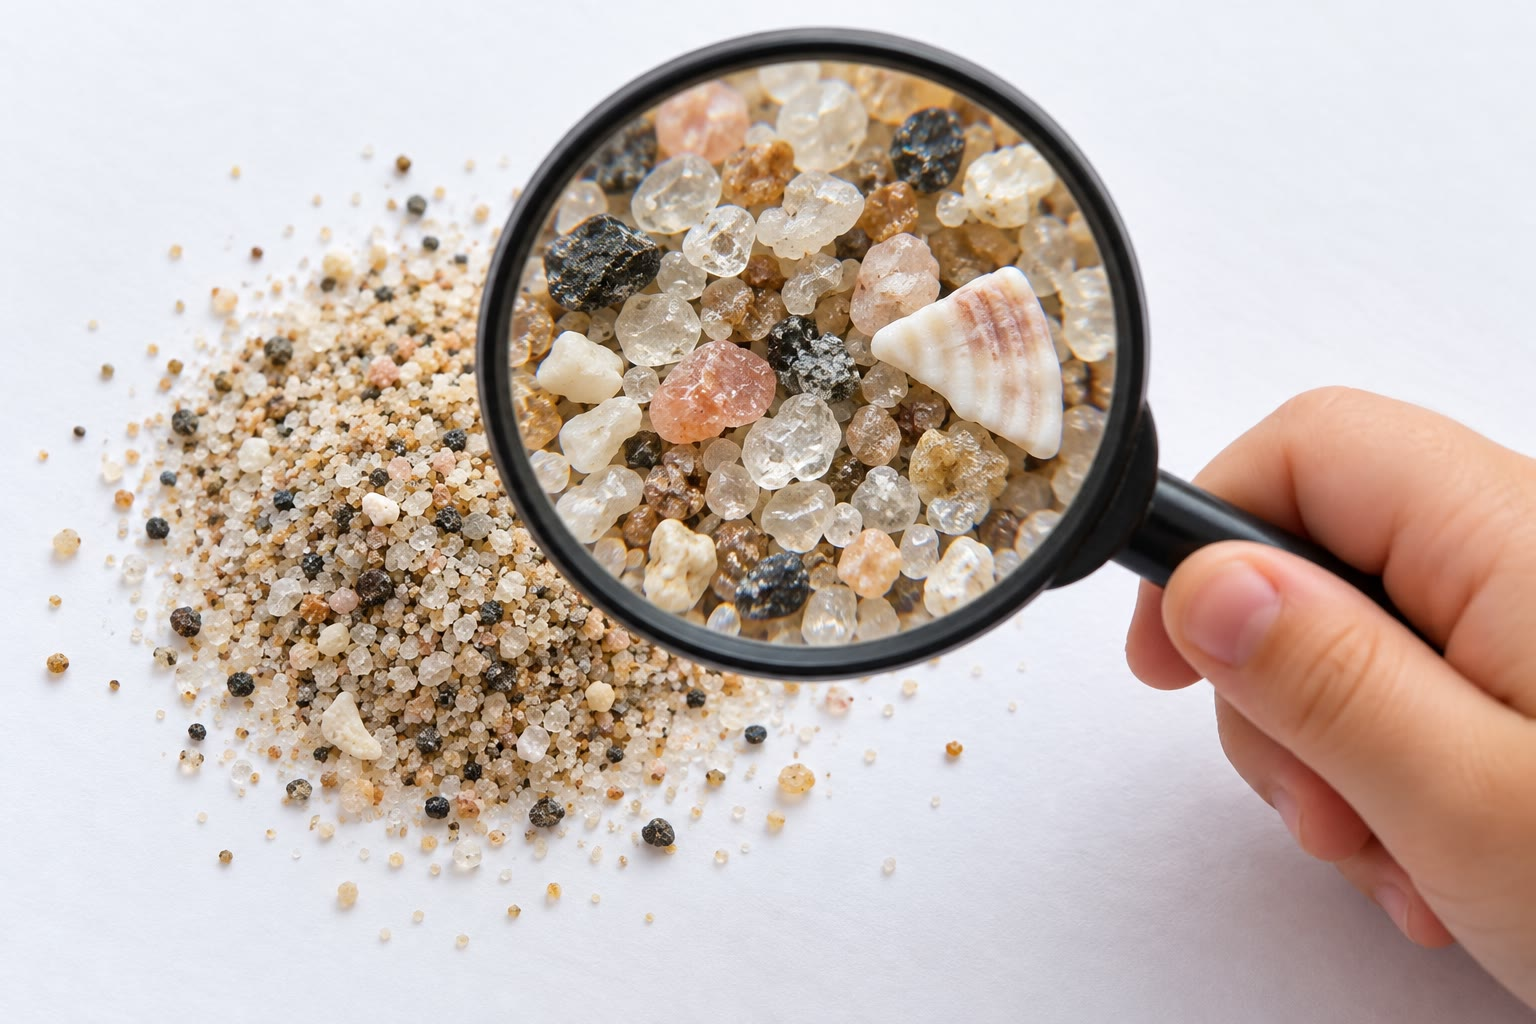
\includegraphics[width=0.55\linewidth]{images/book1/ai/g3-sand-magnifier.jpg}

{\small 用放大镜看海滩沙：细小的\omterm{def:g3:stones-pebbles-sand:rock}{岩石}颗粒
和贝壳碎片。}
\end{omfigure}

\begin{method}[按大小给碎岩石分类]\label{met:g3:stones-pebbles-sand:sort}
要给一块碎\omterm{def:g3:stones-pebbles-sand:rock}{岩石}命名，先看它的大小：
\begin{enumerate}
  \item 即使凑近看也分不清颗粒，它是泥；
  \item 能看清每一粒，但每粒都小于 2
        毫米（约一枚硬币的厚度），它是沙；
  \item 若碎块比这更大，但能用手拿起，
        它是\omterm{def:g3:stones-pebbles-sand:pebble}{砾石}或\omterm{def:g3:stones-pebbles-sand:pebble}{卵石}；
  \item 若碎块重得抬不起来，它是巨砾。
\end{enumerate}
\end{method}

\begin{example}[各种大小的碎屑分别在哪里找到？]\label{ex:g3:stones-pebbles-sand:where}
流速快的水能搬运大石块；流速慢的水会把它们留下，只搬运
细小颗粒。因此，巨砾和棱角分明的石块位于陡峭的山间
溪流中；\omterm{def:g3:stones-pebbles-sand:pebble}{卵石}和\omterm{def:g3:stones-pebbles-sand:pebble}{砾石}位于\omterm{def:g1:landscapes-around-us:landform}{山谷}中\omterm{def:g1:landscapes-around-us:water}{河流}的岸边；
沙聚集在海滩和\omterm{def:g1:landscapes-around-us:water}{河流}平静的弯道处；泥则沉积在
水几乎静止的地方，如池塘、\omterm{def:g1:landscapes-around-us:water}{湖泊}和河口。
\end{example}

\section{硬岩石与软岩石}

并非所有\omterm{def:g3:stones-pebbles-sand:rock}{岩石}都同样坚硬。有些\omterm{def:g3:stones-pebbles-sand:rock}{岩石}，如花岗岩，非常坚硬，以至
能划伤玻璃，在墙体中可保存数千年。另一些\omterm{def:g3:stones-pebbles-sand:rock}{岩石}在
手中一捏即碎，如白垩，它能在黑板上留下白色痕迹。还有些\omterm{def:g3:stones-pebbles-sand:rock}{岩石}
由肉眼可见的颗粒组成；另一些则很光滑，从这一面到那一面看上去
都一样。

\begin{example}[三种岩石的比较]\label{ex:g3:stones-pebbles-sand:three}
\emph{花岗岩}布满粉色、白色和黑色的颗粒，非常
坚硬。\emph{砂岩}由\omterm{def:g3:stones-pebbles-sand:sand}{沙粒}胶结而成；用手指
摩擦时，有时会掉下几粒沙。\emph{白垩}呈白色，
质地柔软、呈粉末状。你将在以后的年级学习它们各自是如何
形成的。
\end{example}

\begin{omfigure}
\begin{tikzpicture}[font=\small]
  % three stones seen through a magnifying glass (drawn, not to scale)
  % granite: interlocking grains of three colours
  \begin{scope}
    \clip (0,0) circle (1.5);
    % a jittered lattice: the cells tile the disk with no gap, like the
    % interlocking crystals of granite
    \foreach \i in {-6,...,5} \foreach \j in {-6,...,5} {
      \pgfmathtruncatemacro{\c}{mod(abs(37*\i+17*\j+\i*\j),7)}
      \ifcase\c \def\col{pink!70}\or\def\col{pink!45}\or\def\col{white}\or
        \def\col{black!12}\or\def\col{white}\or\def\col{black!80}\else\def\col{pink!60}\fi
      \fill[\col, draw=black!35, line width=0.3pt]
        ({0.27*\i+0.07*sin(90*\i+131*\j)},{0.27*\j+0.07*cos(77*\i+61*\j)}) --
        ({0.27*(\i+1)+0.07*sin(90*(\i+1)+131*\j)},{0.27*\j+0.07*cos(77*(\i+1)+61*\j)}) --
        ({0.27*(\i+1)+0.07*sin(90*(\i+1)+131*(\j+1))},{0.27*(\j+1)+0.07*cos(77*(\i+1)+61*(\j+1))}) --
        ({0.27*\i+0.07*sin(90*\i+131*(\j+1))},{0.27*(\j+1)+0.07*cos(77*\i+61*(\j+1))}) -- cycle;
    }
  \end{scope}
  \draw[black!70, line width=2pt] (0,0) circle (1.5);
  \node at (0,-1.9) {花岗岩};
  \node[font=\scriptsize, align=center] at (0,-2.45) {三种颜色的大颗粒，\\彼此紧密咬合};
  % sandstone: rounded grains touching
  \begin{scope}[xshift=4.2cm]
    \clip (0,0) circle (1.5);
    \fill[brown!45] (-1.6,-1.6) rectangle (1.6,1.6);
    \foreach \x in {-1.5,-1.1,...,1.6} \foreach \y in {-1.5,-1.15,...,1.6}
      \fill[yellow!50!brown!70, draw=brown!70!black, line width=0.3pt]
        ({\x+0.08*sin(97*\x+61*\y)},{\y+0.07*cos(53*\x-89*\y)}) circle ({0.16+0.03*sin(71*\x*\y)});
  \end{scope}
  \draw[black!70, line width=2pt] (4.2,0) circle (1.5);
  \node at (4.2,-1.9) {砂岩};
  \node[font=\scriptsize, align=center] at (4.2,-2.45) {圆润的沙粒 \\胶结在一起};
  % chalk: smooth, no grains to see
  \begin{scope}[xshift=8.4cm]
    \fill[white] (0,0) circle (1.5);
  \end{scope}
  \draw[black!70, line width=2pt] (8.4,0) circle (1.5);
  \node at (8.4,-1.9) {白垩};
  \node[font=\scriptsize, align=center] at (8.4,-2.45) {白色且光滑：颗粒 \\太小，看不见};
\end{tikzpicture}

{\small 用放大镜观察的三块\omterm{def:g3:stones-pebbles-sand:rock}{岩石}（图中为示意）。花岗岩和砂岩的
颗粒清晰可见；白垩在各处看起来都一样。}
\label{fig:g3:stones-pebbles-sand:magnified}
\end{omfigure}

\begin{method}[仔细观察一块石头]\label{met:g3:stones-pebbles-sand:look}
要描述一块石头，请在不把它弄碎的前提下，看一看它，摸一摸它：
\begin{enumerate}
  \item 它的颜色，或它的几种颜色；
  \item 它的形状：有棱角，还是圆润光滑；
  \item 它的颗粒：能看见吗？颗粒是否都一样，还是有几种
        颜色？
  \item 它的手感：坚硬，还是软到能在纸上留下痕迹？
\end{enumerate}
把看到的内容写在表格里，每块石头占一行。
\end{method}

\begin{example}[三块石头的表格]\label{ex:g3:stones-pebbles-sand:table}
米娅描述了学校盒子里的三块石头。
\begin{center}\small
\begin{tabular}{llll}
\hline
石头 & 颜色 & 形状 & 颗粒 \\
\hline
A & 粉色、白色和黑色 & 圆润 & 大，三种颜色 \\
B & 黄褐色 & 有棱角 & 小，颜色都一样 \\
C & 白色 & 有棱角 & 看不见 \\
\hline
\end{tabular}
\end{center}
石头 C 还会在纸上留下白色痕迹。由上面的例子可知，石头 A
像花岗岩，石头 B 像砂岩，石头 C 像白垩。石头 A
是圆的：水流长时间冲刷使它变圆。
\end{example}

\section{我们建造所用的石材}

几千年来，人们一直就地取用周围的\omterm{def:g3:stones-pebbles-sand:rock}{岩石}来建造房屋。在
某个地区的古老村庄里，墙壁往往是同一种颜色，
因为它们是用附近山丘上的石头建成的。

\begin{definition}[建筑石材]\label{def:g3:stones-pebbles-sand:building-stone}
\emph{建筑石材}\index{建筑石材}是指经过切割或加工，
用来砌墙、盖屋顶、做台阶、建桥或铺路的\omterm{def:g3:stones-pebbles-sand:rock}{岩石}。
\end{definition}

每种\omterm{def:g3:stones-pebbles-sand:rock}{岩石}都有各自的用处。坚硬的花岗岩可以用来砌墙、做台阶和
路缘石，能用上几个世纪。有些\omterm{def:g3:stones-pebbles-sand:rock}{岩石}，比如板岩，会裂成又薄又平的
石片：一片压着一片铺上去，
就能做成挡雨的屋顶。砂岩和石灰岩足够软，可以切成整齐的石块。

\begin{omfigure}
\begin{minipage}[b]{0.49\linewidth}\centering
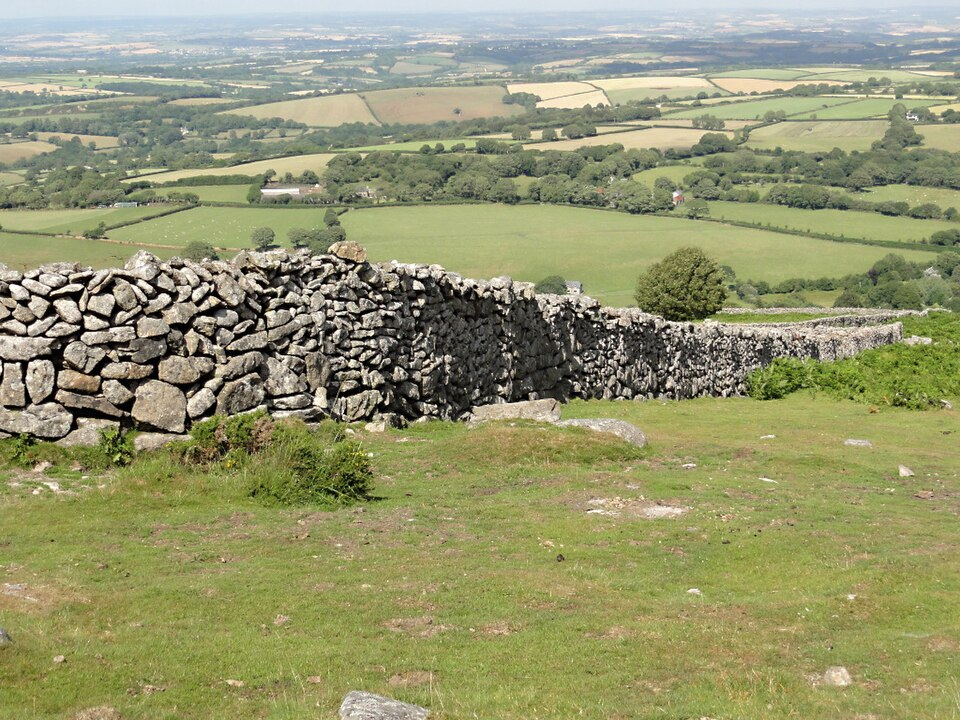
\includegraphics[width=\linewidth]{images/book1/g3-granite-wall.jpg}

{\small 由花岗\omterm{def:g3:stones-pebbles-sand:rock}{岩石}块砌成、未用砂浆的墙。照片：Tony
Atkin, Geograph（CC BY-SA 2.0）。}
\end{minipage}\hfill
\begin{minipage}[b]{0.49\linewidth}\centering
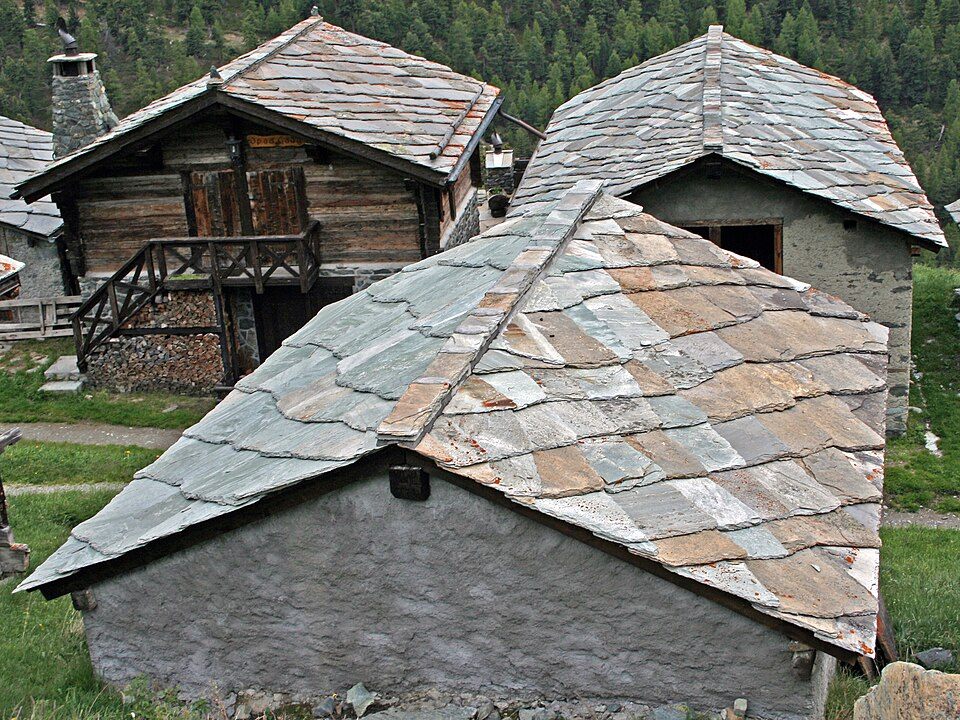
\includegraphics[width=\linewidth]{images/book1/g3-slate-roof.jpg}

{\small 瑞士山村中用薄而平的石板盖成的屋顶。
照片：Michael C. Rygel（CC BY-SA 3.0）。}
\end{minipage}
\end{omfigure}

\begin{omfigure}
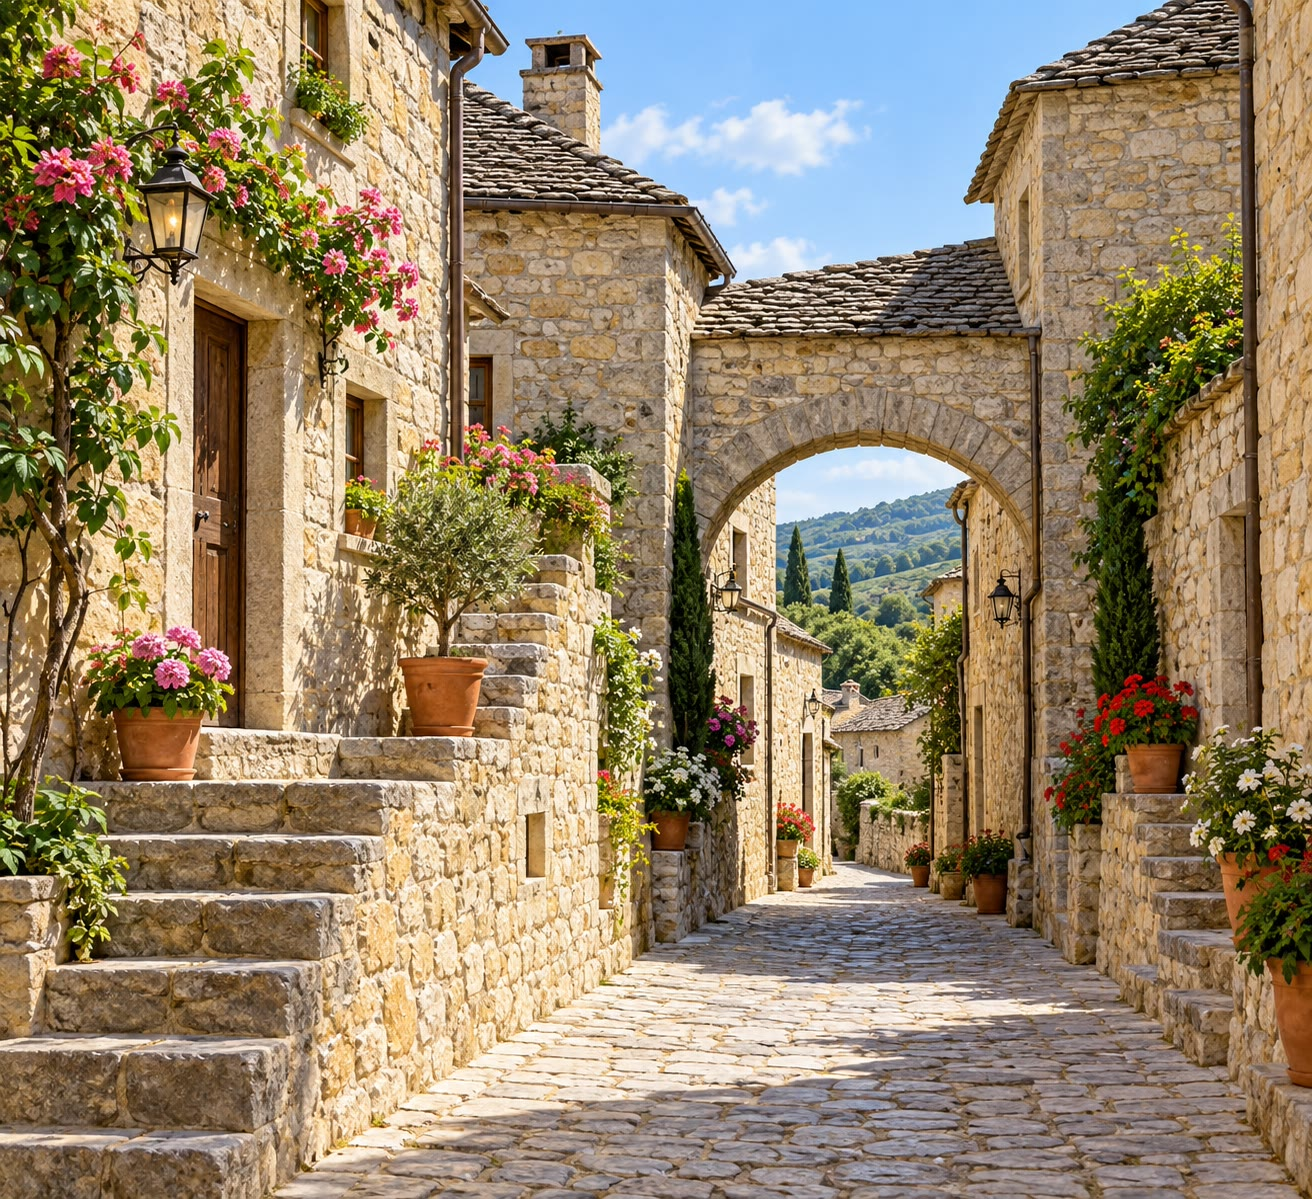
\includegraphics[width=0.6\linewidth]{images/book1/ai/g3-stone-village.jpg}

{\small 一座完全用附近山丘上的石头建成的古老村庄。}
\end{omfigure}

今天，我们还用砖、混凝土和玻璃来建造。但砖是用
烧制的黏土做成的，混凝土由沙、\omterm{def:g3:stones-pebbles-sand:pebble}{砾石}和水泥制成，玻璃则
由沙制成：它们归根结底也都来自地球上的\omterm{def:g3:stones-pebbles-sand:rock}{岩石}。

\section{练习}

\begin{exercise}[$\star$]\label{exo:g3:stones-pebbles-sand:1}
什么是\omterm{def:g3:stones-pebbles-sand:rock}{基岩}？不挖掘的话，在哪里可以看到它？
\end{exercise}

\begin{exercise}[$\star$]\label{exo:g3:stones-pebbles-sand:2}
按大小排序，从小到大：\omterm{def:g3:stones-pebbles-sand:pebble}{卵石}、泥、
巨石、沙。
\end{exercise}

\begin{exercise}[$\star$]\label{exo:g3:stones-pebbles-sand:3}
一颗颗粒的直径为 1 毫米。它是沙还是\omterm{def:g3:stones-pebbles-sand:pebble}{砾石}？另一颗颗粒的
直径为 3 毫米：它是沙还是\omterm{def:g3:stones-pebbles-sand:pebble}{砾石}？
\end{exercise}

\begin{exercise}[$\star$]\label{exo:g3:stones-pebbles-sand:4}
天然的还是人造的？一颗\omterm{def:g3:stones-pebbles-sand:pebble}{卵石}；一块砖；一块花岗\omterm{def:g3:stones-pebbles-sand:rock}{岩石}块；一片
玻璃；海滩上的沙。
\end{exercise}

\begin{exercise}[$\star$]\label{exo:g3:stones-pebbles-sand:5}
为什么河里的\omterm{def:g3:stones-pebbles-sand:pebble}{卵石}没有尖锐的棱角？
\end{exercise}

\begin{exercise}[$\star$]\label{exo:g3:stones-pebbles-sand:6}
说出两种\omterm{def:g3:stones-pebbles-sand:building-stone}{建筑石材}，并指出它们在
本章照片中各自的用途。
\end{exercise}

\begin{exercise}[$\star\star$]\label{exo:g3:stones-pebbles-sand:7}
汤姆找到两块同一种\omterm{def:g3:stones-pebbles-sand:rock}{岩石}的石头：一块有棱角，另一块是圆的。
哪一块被搬运的距离更远？请说明理由。
\end{exercise}

\begin{exercise}[$\star\star$]\label{exo:g3:stones-pebbles-sand:8}
在颗粒大小示意图上，最大的\omterm{def:g3:stones-pebbles-sand:pebble}{卵石}有多少厘米长？
沿 1 厘米的长度，能并排放下多少颗
直径为 2 毫米的\omterm{def:g3:stones-pebbles-sand:sand}{沙粒}？
\end{exercise}

\begin{exercise}[$\star\star$]\label{exo:g3:stones-pebbles-sand:9}
你觉得在哪里最可能找到泥：是在湍急的山间溪流中，还是在
安静的池塘里？为什么？
\end{exercise}

\begin{exercise}[$\star\star$]\label{exo:g3:stones-pebbles-sand:10}
砖、混凝土和玻璃都是人造的。为什么我们仍然可以说
它们来自地球上的\omterm{def:g3:stones-pebbles-sand:rock}{岩石}？
\end{exercise}
